\def\mytitle{CIRCLE}
\def\myauthor{VAMSI SUNKARI}
\def\contact{vamsisunkari9849@gmail.com}
\def\mymodule{Future Wireless Communication (FWC)}
\documentclass[10pt, a4paper]{article}
\usepackage[a4paper,outer=1.5cm,inner=1.5cm,top=1.75cm,bottom=1.5cm]{geometry}
\twocolumn
\usepackage{setspace}
\usepackage{graphicx}
\graphicspath{{./images/}}
\usepackage[colorlinks,linkcolor={black},citecolor={blue!80!black},urlcolor={blue!80!black}]{hyperref}
\usepackage[parfill]{parskip}
\usepackage{lmodern}
\usepackage{tikz}
 \usepackage{physics}
%\documentclass[tikz, border=2mm]{standalone}
\usepackage{karnaugh-map}
\usepackage{tabularx}
\usetikzlibrary{calc}
\usepackage{amsmath}
\usepackage{amssymb}
\renewcommand*\familydefault{\sfdefault}
\usepackage{watermark}
\usepackage{lipsum}
\usepackage{xcolor}
\usepackage{listings}
\usepackage{float}
\usepackage{titlesec}
\providecommand{\mtx}[1]{\mathbf{#1}}
\titlespacing{\subsection}{1pt}{\parskip}{3pt}
\titlespacing{\subsubsection}{0pt}{\parskip}{-\parskip}
\titlespacing{\paragraph}{0pt}{\parskip}{\parskip}
\newcommand{\figuremacro}[5]{//
    \begin{figure}[#1]
        \centering
        \includegraphics[width=#5\columnwidth]{#2}
        \caption[#3]{\textbf{#3}#4}
        \label{fig:#2}
    \end{figure}
}
\newcommand{\myvec}[1]{\ensuremath{\begin{pmatrix}#1\end{pmatrix}}}
\let\vec\mathbf
\lstset{
frame=single, 
breaklines=true,
columns=fullflexible
}

\title{\mytitle}
\author{\myauthor\hspace{1em}\\\contact\\FWC22040\hspace{6.5em}IITH\hspace{0.5em}\mymodule\hspace{6em}ASSIGN-5}
\date{}
\begin{document}
 \maketitle
 \tableofcontents
 \section{Problem}
 Let a circle be given by $2x(x-a)+y(2y-a)=0 (a\neq0, b\neq0) $. Find the condition    on  a and b  if two chords each bisected by the x-axis, can be drawn to the circle from $\myvec{a\\ \frac{b}{2}}$
 \section{Construction}
 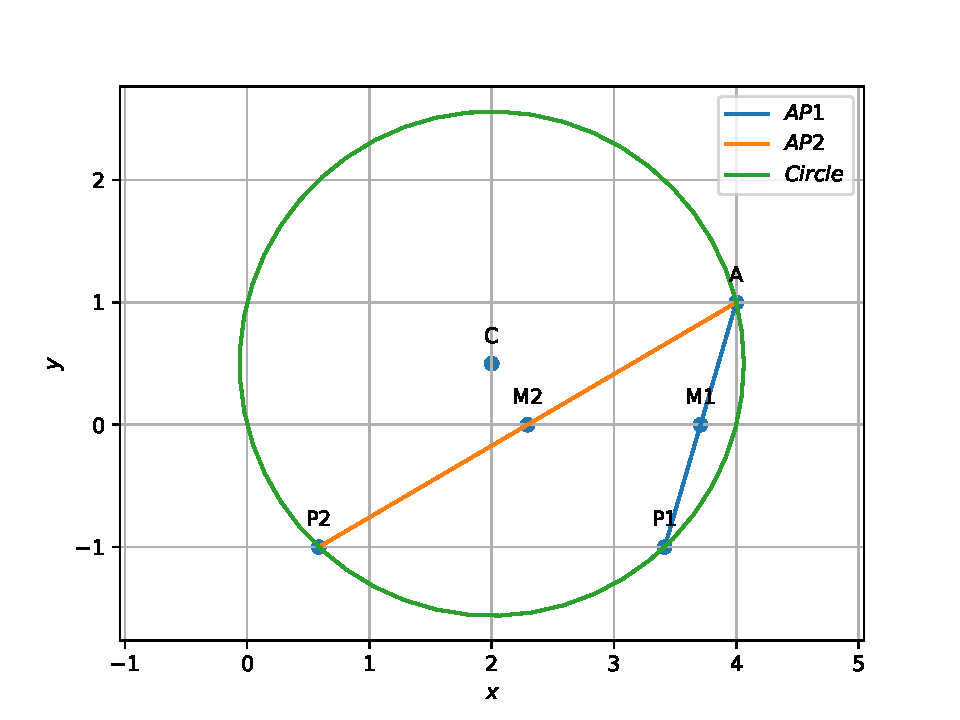
\includegraphics[scale=0.5]{par.pdf}
 \section{Solution}
 \begin{center}
 \subsection{Considerations}
 \begin{tabular}{|c|c|}
 \hline
 \textbf{Symbol}&\textbf{Value}\\
 \hline
 a&4\\
 \hline
 b&2\\
 \hline
\end{tabular}\\
\ 
\\
\end{center}
\begin{center}
The given circle is 
\begin{equation}
	\vec{X}^T\vec{V}\vec{X} + 2\vec{u}^T\vec{X} + f = 0
\end{equation}
\begin{center}
    $\vec{V} = \vec{I}$ \\
    $\vec{u} = \myvec{\frac{-a}{2} \\ \frac{-b}{4}}$\\
    $f=0$
\end{center}
\end{center}

\subsection{Part 1:}
let $\vec{P_1}$ and $\vec{P_2}$ be the other points of the chord. So, they satisfy the circle equation.
\begin{equation}
    \vec{P_1}^T\vec{P_1} + 2\vec{u}^T\vec{P_1}  = 0
\end{equation}
\begin{equation}
     \vec{P_2}^T\vec{P_2} + 2\vec{u}^T\vec{P_2} = 0
\end{equation}
$\vec{\frac{A+P_1}{2}}$ and $\vec{\frac{A+P_2}{2}}$ are the midpoints of the chords and lies on 
\begin{equation}
    e_2^T\vec{x} = 0
\end{equation}
so,
\begin{equation}
    e_2^T(\vec{\frac{A+P_1}{2}}) = 0
\end{equation}
\begin{equation}
    e_2^T(\vec{\frac{A+P_2}{2}}) = 0
\end{equation}
\begin{equation}
    \myvec{0 & 1}\myvec{x+a \\ y+\frac{b}{2}} = 0
\end{equation}

\begin{equation}
    y = -\frac{b}{2}
\end{equation}
The other point is $\myvec{x\\ -\frac{b}{2}}$  which satisfies the parabola equation.
\begin{equation}
	\myvec{x & -\frac{b}{2}}\myvec{x \\ -\frac{b}{2}} +2\myvec{\frac{-a}{2} & \frac{-b}{4}}\myvec{x \\ -\frac{b}{2}}  = 0
\end{equation}
\begin{equation}
    x^2 - ax + \frac{b^2}{2} = 0
\end{equation}
The solution of above equation gives the x coordinates of the points
\begin{equation}
    x = \frac{a \pm \sqrt{a^2 - 2b^2}}{2}
\end{equation}
\subsection{Part 2}
It is clear that there are two distinct points on the X-axis.
$\therefore$ the discriminant of quadratic equation is positive\\
\begin{equation}
    \implies \Delta > 0
\end{equation}
\begin{equation}
    {a^2 - 2b^2} > 0
\end{equation}
\begin{equation}
a^2 > 2b^2
\end{equation}
The condition on a and b if two chords each bisected by the x-axis, can be drawn to the circle from $\myvec{a \\ \frac{b}{2}}$ is 
$a^2 > 2b^2$





if $a^2=2b^2$  condition is violated then x-axis bisects only 1 chord


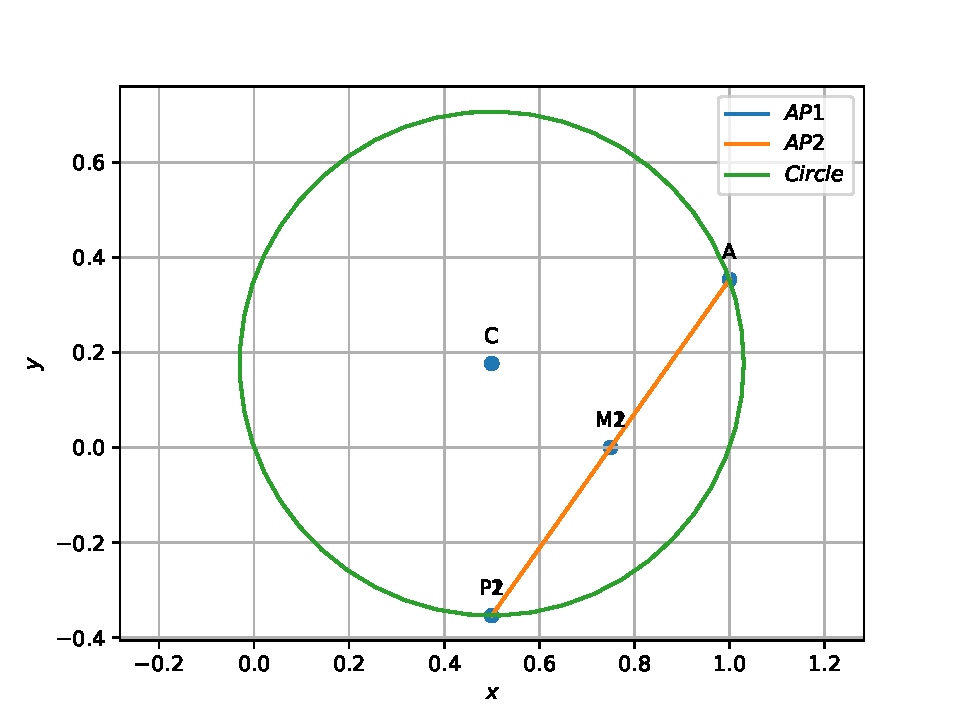
\includegraphics[scale=0.5]{para.pdf}



if $a^2<2b^2$  the conditon is violated roots are imaginary and it is not possible to draw chords 

\end{document}
